\documentclass[nonumber]{homework}
\usepackage{enumitem}

\newcommand{\hwclass}{Math 6108}
\newcommand{\hwname}{Jacob Hauck}
\newcommand{\hwtype}{Homework}

\newcommand{\R}{\textbf{R}}
\newcommand{\dee}{\;\text{d}}
\newcommand{\eps}{\varepsilon}
\newcommand{\pl}[2]{\frac{\partial #1}{\partial #2}}
\newcommand{\dl}[2]{\frac{\text{d} #1}{\text{d} #2}}
\newcommand{\sgn}{\text{sgn}}
\newcommand{\bigoh}{\mathcal{O}}

\newcommand{\hwnum}{10}


\begin{document}
	\maketitle
	
	\question*{7.8(b)}
	
	Consider the product system
	\begin{equation*}
		\dot{x}_1 = x_1^2, \qquad \dot{x}_2 = -x_2.
	\end{equation*}
	Solving each equation, we have $x_2 = x_2(0)e^{-t}$, and $x_1 = \frac{x_1(0)}{1-x_1(0) t}$ if $x_1(0)\ne0$, and $x_1 = 0$ if $x_1(0) = 0$. Therefore, the maximal interval of existence is 
	\begin{equation*}
		I = \begin{cases}
			(-\infty, 1/x_1(0))& x_1(0) > 0,\\
			 (-\infty, \infty) & x_1(0) = 0, \\
			 (1/x_1(0), \infty) & x_1(0) < 0.
			\end{cases}
	\end{equation*}
	From the solution formulas we have
	\begin{equation*}
		\lim_{t\to \infty} x_2 = 0,
	\end{equation*}
	and
	\begin{equation*}
		\lim_{t\to-\infty}x_2 = \begin{cases}
			\infty & x_2(0) > 0, \\
			0 & x_2(0) = 0,\\
			-\infty & x_2(0) < 0.
		\end{cases}
	\end{equation*}
	We also have
	\begin{align*}
		\lim_{t\to 1/x_1(0)^-} x_1 &= \infty \qquad \text{ if } x_1(0) > 0,\\
		\lim_{t\to\infty} x_1 &= 0 \qquad \text{ if } x_1(0) < 0,
	\end{align*}
	and
	\begin{align*}
		\lim_{t\to -\infty} x_1 &= 0 \qquad \text{ if } x_1(0) > 0,\\
		\lim_{t\to 1/x_1(0)^+} x_1 &= -\infty \qquad \text{ if } x_1(0) < 0.
	\end{align*}
	
	If $x_2 \ne0$ and $x_1\ne0$, then we have
	\begin{equation*}
		\frac{\text{d}x_1}{\text{d}x_2} = -\frac{x_1^2}{x_2} \implies -\frac{\text{d}x_1}{x_1^2} = \frac{\text{d}x_2}{x_2} \implies \frac{1}{x_1} = \ln|x_2| + C,
	\end{equation*}
	for some constant $C$, or, equivalently,
	\begin{equation*}
		x_2 = Ae^\frac{1}{x_1},
	\end{equation*}
	for some constant $A \ne0$.
	
	If $x_1(0) < 0$, then $x_1 \to 0$ from the left as $t \to \infty$, so $x_2 \to 0$, and $(x_1,x_2) \to (0,0)$. If $x_1(0) > 0$, then $x_1 \to \infty$ as $t\to 1/x_1(0)$, so $x_2 \to x_2(0)e^{-1/x_1(0)}$ as $t\to 1/x_1(0)$. Additionally, if $x_1(0) <0$, then $x_1 \to  -\infty$ as $t \to 1/x_1(0)$, and if $x_1(0) > 0$, then $x_1 \to 0$ from the right as $t\to- \infty$, so $x_2 \to \infty$ as $t \to -\infty$.
	
	These considerations result in the phase plane diagram in Figure \ref{fig:78b}.
	\begin{figure}[h]
		\centering
		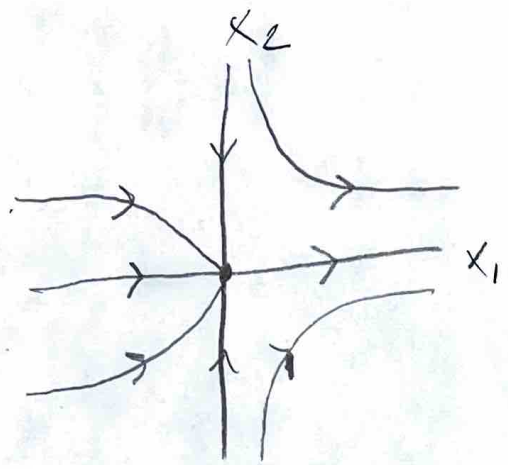
\includegraphics[width=.6\textwidth]{p78b.png}
		\caption{7.8(b) Phase portrait}
		\label{fig:78b}
	\end{figure}
	Furthermore, the $\omega$-limit and $\alpha$-limit sets are given by
	\begin{align*}
		\omega(x_1(0),x_2(0)) &= \begin{cases}
			\{(0,0)\} & x_1(0) \le 0 \\
			\varnothing & x_1(0) > 0,
		\end{cases}\\[0.5em]
		\alpha(x_1(0), x_2(0)) &= \begin{cases}
			\{(0,0)\} & x_1(0)\ge 0 \text{ and } x_2(0) = 0, \\
			\varnothing & \text{otherwise}.
		\end{cases}
	\end{align*}
	
	\question*{7.8(c)}
	
	Consider the product system
	\begin{equation*}
		\dot{x}_1 = -x_1, \qquad \dot{x}_2 = x_2 -x_2^3.
	\end{equation*}
	Then $x_1 = x_1(0)e^{-t}$, and the asymptotic behavior of $x_2$ is determined by the phase line diagram in Figure \ref{fig:78c_pld}. Based on these facts, we obtain the phase portrait in Figure \ref{fig:78c}.
	\begin{figure}[h]
		\centering
		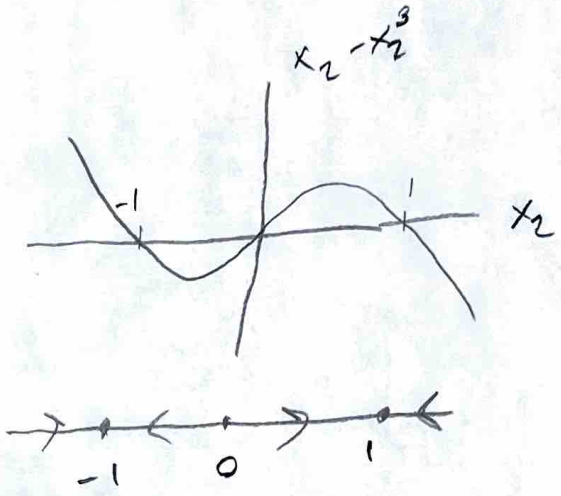
\includegraphics[width=.6\textwidth]{p78c_pld.png}
		\caption{Phase line diagram for $x_2$ equation}
		\label{fig:78c_pld}
	\end{figure}
	\begin{figure}[h]
		\centering
		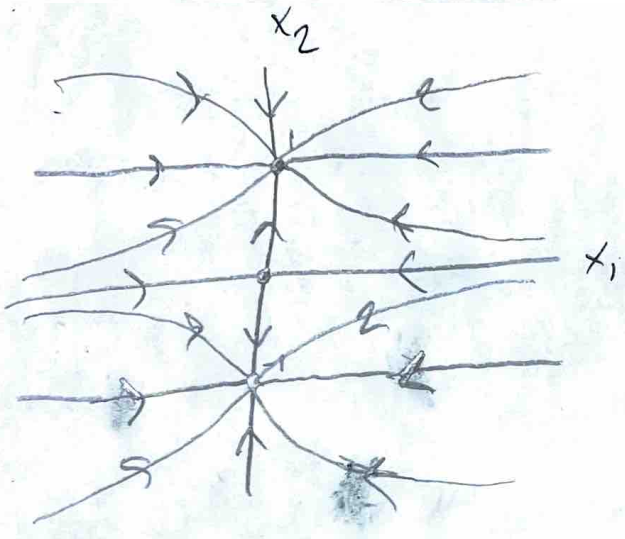
\includegraphics[width=.6\textwidth]{p78c.png}
		\caption{7.8(c) Phase portrait}
		\label{fig:78c}
	\end{figure}
	Finally, we can determine the $\alpha$-limit and $\omega$-limit sets from the phase portrait:
	\begin{align*}
		\omega(x_1(0), x_2(0)) &= \begin{cases}
			(0,0) & x_2(0) = 0, \\
			(0,1) & x_2(0) > 0, \\
			(0, -1) & x_2(0) < 0
		\end{cases}\\[0.5em]
		\alpha(x_1(0), x_2(0)) &= \begin{cases}
			(0,0) & x_1(0) = 0 \text{ and } |x_2(0)| < 1, \\
			\varnothing & \text{otherwise}.
		\end{cases}
	\end{align*}
	
\end{document}